%\documentclass{article}
\documentclass[a4paper, 12pt, oneside]{book} % Uses the book template for quick start, but scrbook may be better because it is more flexible
\usepackage{inputenc}
\emergencystretch=2em
\usepackage[breaklinks]{hyperref}
\hypersetup{
    colorlinks=true,
    linkcolor=blue,
    filecolor=magenta,      
    urlcolor=magenta,
    citecolor=black}
\usepackage[english]{babel}
%\usepackage{biblatex}
\usepackage[backend=biber, style=apa]{biblatex}
\setlength\bibitemsep{\baselineskip}
\usepackage{svg}
\usepackage{graphicx}
\usepackage[labelfont=bf]{caption}
\usepackage[left]{lineno} % For line numbers
%\renewcommand{\baselinestretch}{2.0}
%\linenumbers
\usepackage[T1]{fontenc} % Include italic fonts
\usepackage{geometry} % Page margins
\usepackage{titling} % Title page container
\usepackage{wrapfig} % Picture container
\usepackage{titlesec} % Remove chapter header
\renewcommand{\familydefault}{\sfdefault} % Set default f
\usepackage{comment}

% COLORS
%\usepackage{xcolor} 
%\usepackage{soul}
%\definecolor{color1}{HTML}{a5ddd0}
%\definecolor{color2}{HTML}{00441b}
%\sethlcolor{color1}\hl{Its trunk bears spikes to deter attacks by animals. <0.35> }
%\sethlcolor{color2}\hl{Branches usually in whorls of 3. <1.0> }

\addbibresource{references.bib}
% Note: Fill these in with correct data, they are used throughout the document
\title{A Step Towards Explainable AI: Infer Species Names Based on Partial Descriptions in Natural Language}
\author{Robert van de Vlasakker}
% This can be left as-is to automatically update
\date{\today}
\geometry{top=2.25cm, 
            bottom=2.91cm,
            inner=2.91cm,
            outer=2.91cm,
            foot=0cm,
            includeheadfoot} % First page margins
\titleformat{\chapter}[display]
  {\normalfont\bfseries}{}{0pt}{\Large}

\begin{document}
 \begin{titlingpage}


  %\newgeometry{top=1.25cm,bottom=1.25cm,inner=0.66cm,outer=0.53cm,foot=1.19cm,includeheadfoot} % Subsequent page margins
  % Note: this uses the MS Word template margins, you might want to increase them a bit for printing (e.g. inner=1.91cm,outer=1.91cm)
  \thispagestyle{empty}
  
  \begin{center}
  {\bfseries \Large \thetitle}
  \newline
  \newline
  \newline
  \newline
  %{\bfseries \itshape Subtitle}\vspace{2.7cm}
  
  {\Large \theauthor}\vspace{0.8cm}
  
  {Registration number 920523897020}\vspace{2.5cm}
  
  {\large \underline{Supervisors}:}\vspace{1.1cm}
  
  {Diego Marcos}
  
  {Ioannis Athanasiadis}\vspace{3.0cm}
  
  %{A thesis submitted in partial fulfilment of the degree of Master of Science}
  
  %{at Wageningen University and Research Centre,}
  
  %{The Netherlands.}\vspace{2.7cm}
  \end{center}
  
  \begin{center}
    {\thedate}
  
    {Wageningen, The Netherlands}
  \end{center}\vspace{6cm}

    Thesis code number: GRS-80400
  
    Thesis Report: Proposal
  
    {Wageningen University and Research Centre}
  
    {Laboratory of Geo-Information Science and Remote Sensing}
 \end{titlingpage}
\graphicspath{ {./figures/} }

\renewcommand{\thesection}{\arabic{section}}


\section{Introduction}
Estimated is that 50\% of the species are yet to be discovered, and many species will go extinct before ever being described \autocite{lees_species_2015}.
Scalable technologies that can help monitor diversity and help discover new species are more needed than ever.
Deep neural networks (DNNs) can help discover new species, automate and speed up this process \autocite{van_horn_inaturalist_2018}.
However, DNNs are quite rigid, and their black-box behaviour could raise issues as it hampers the trustworthiness of the models \autocite{carvalho_machine_2019}.
%However, DNNs are quite rigid and often act as black boxes.
%We first need to learn DNNs to reason like taxonomists. 
It is essential to get more insights into the reasoning of a deep learning model in sensitive fields like taxonomy.
This way, we can learn a DNN to reason like an experienced taxonomist when describing existing and new species.

Deep neural networks (DNNs) allow for remarkable performance in applications: from the automatic classification of text and images, natural language processing (NLP), to reinforcement learning.
DNNs outperform most classic machine learning approaches \autocite{he_delving_2015, brown_language_2020}.
The key to their success is end-to-end training.
Unlike classic machine learning models, deep learning models can automatically extract features needed for detection or classification.
Domain knowledge, in combination with careful engineering to extract the necessary features for the detection or classification, is no longer needed \autocite{lecun_deep_2015}.
However, end-to-end training also results in DNNs that are rigid, difficult to interpret and explain.

%Because the networks parameters are updated based on its input data, the reasoning of DNNs remains challenging to understand \autocite{li_interpretable_2021, losch_interpretability_2019} and they do not perform well on long-tailed datasets, like most real-real world dataset \autocite{van_horn_inaturalist_2018}.
%This limits their capabilities in automatic classification of species.
%When the reason behind DNNs' behaviour is better understood, the insights could improve their performance \autocite{amershi_modeltracker_2015}.% and the models can be expanded to more fields \autocite{lei_opening_2018}.

%Unlike classic machine learning models, deep learning models can automatically extract features needed for detection or classification.
%Domain knowledge, in combination with careful engineering to extract the necessary features for the detection or classification, is no longer needed \autocite{lecun_deep_2015}.
To extract the features from the input data, deep learning models use multiple neurons that take the input, process it to a slightly more abstract representation and pass it through the next layer of neurons \autocite{schmidhuber_deep_2015}.
Provided enough layers are stacked upon each other, very complex features can be extracted and correctly detected or classified by such a network.
%However, this means that well represented classes' features are extracted more, then less represented classes. 
Because the network's parameters are updated based on its input data, the reasoning of DNNs remains challenging to understand \autocite{li_interpretable_2021, losch_interpretability_2019}, and they do not perform well on long-tailed datasets, like most real-world datasets \autocite{van_horn_inaturalist_2018}.
Stacking multiple layers of neurons on top of each other often results in millions of parameters, and all of these neurons use non-linear activation functions that decrease the interpretability of the network.
In long-tailed datasets, the parameters are not well optimised for less represented classes as the neurons cannot extract the necessary features.
While this automatic feature extraction is very convenient, it will become difficult to track models' reasons, and it can hamper performance.

A more explainable, less rigid, artificial intelligence (AI) might be created by extending the concept of the semantic bottleneck layer from \textcite{ishikawa_contextual_2021} and splitting a regular convolution neural network (CNN) for image classification into two separate models that communicate using natural language.
The first model will describe species features present in the image, and the second model will take these descriptions and tries to infer the species (see Figure \ref{fig:intro}).
%This semantic bottleneck layer is an intermediate layer that is intepretable for humans\autocite{bucher_semantic_2019}.
%By splitting a regular classification convolution neural network (CNN) into two parts that communicate using natural language this interpretability and rigidity problem might be solved.
This way, DNNs reasonings for species classification can be tracked, mistakes can be spotted, and the models' performance can be improved.


\section{Motivation}

\begin{figure} [t]
    \centering
    \vspace{0cm}
    \makebox[\textwidth][c]{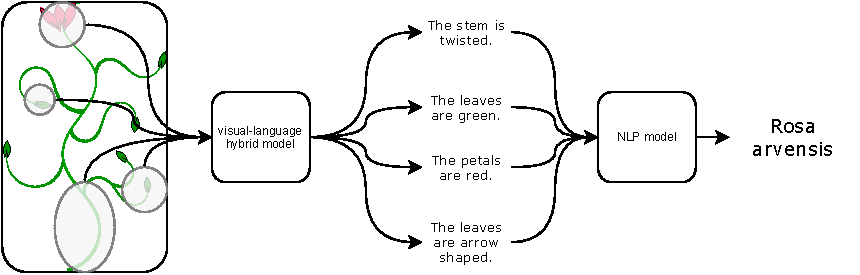
\includegraphics[width=1.25\textwidth]{intrduction_overview.pdf}}
    \caption{The proposed architecture by \textcite{ishikawa_contextual_2021} for species classification. The model input is an image. The first model will describe the attributes present in the image in natural language. The second model will take the output of the first model and will make a prediction. The intermediate results remain interpretable by using natural language.}
    \label{fig:intro}
\end{figure}


Many species look alike.
They are difficult to distinguish, to describe and are easily missclassified.
While DNNs can help automate and improve this classification process, they still rely on large amounts of training samples \autocite{van_horn_inaturalist_2018}.
As most species datasets are long-tailed, these training samples are lacking for many species.
We need a better understanding of an DNN to make it less rigid and more explainable so we can validate and improve the results \autocite{amershi_modeltracker_2015}.

Different algorithms and techniques have been proposed to increase the interpretability of the models.
Common approaches are feature reduction algorithms \autocite{ribeiro_why_2016}, inference of training sample contribution \autocite{koh_understanding_2020}, adding jittering to test samples and see how the prediction changes \autocite{li_understanding_2017} and decomposition and partial derivatives techniques \autocite{samek_explainable_2017}.
These algorithms and techniques all rely on posthoc explanations; they try to interpret an already trained DNN and explain its decisions a posteriori.
They try to identify important features via attributions \autocite{zintgraf_visualizing_2017, selvaraju_grad-cam_2017} or assign meaning to features \autocite{fleet_visualizing_2014}.
While some advances have been made in model understanding, giant leaps forward in the field of explainable AI remain limited \autocite{lipton_mythos_2017, li_interpretable_2021}.
These approaches might explain some of the inner workings of a DNN, but they do not help reason a DNN like a taxonomist, and the intermediate results still remain challenging to interpret. 

An a priori approach entails designing an architecture network with a semantic bottleneck layer that is interpretable for humans \autocite{bucher_semantic_2019}. 
\textcite{ishikawa_contextual_2021} extended this bottleneck layer architecture by training a model that first learns the intermediate results.
First, a model is trained that can predict semantic attributes.
The second model will take the intermediate results to make a final prediction.
By using their architecture, a less rigid, more explainable AI for species classification might be created.

The first model will be a visual-language model that extracts the species attributes from an image and describes its results in natural language. 
This vision hybrid model will be based on the researches of \textcite{radford_learning_2021} and \textcite{huang_interpretable_2020}.
Their findings allow the first model to learn to extract information from images by looking at raw text data that comes with image captions and describe objects present in those images.
This visual-language hybrid model will describe learned species attributes and use zero-shot learning to describe unseen (new) distinctive species attributes.
The second model is a pure natural language processing (NLP) model that takes the partial descriptions and infer the species.
This way, a models reasoning for species predictions might be tracked by investigating the intermediate results \autocite{ishikawa_contextual_2021}.
This allows taxonomists to track a model's reason for predicting an existing species or predicting a not yet discovered species.

For the training of both models, an extensive labelled database with species and their descriptions is needed. 
Unfortunately, such a database does not yet exist and needs to be created for this research to happen.
This dataset needs as many unique descriptions as possible for each species, so for both a taxonomist and the NLP model, it would be possible to infer the species name based on provided descriptions.
The NLP model needs to make predictions on partial descriptions, but in the meantime, it should be clear which parts of the description data is used to make to prediction so the reasoning can be evaluated.
This research will focus on creating and curating the dataset containing species and their descriptions and the training and evaluation of the NLP model.

% OLD STUFF
\begin{comment}
Deep neural networks (DNNs) allow for remarkable performance in applications: from the automatic classification of text and images, natural language processing (NLP) to reinforcement learning.
DNNs outperform most classic machine learning approaches \autocite{he_delving_2015, brown_language_2020}.
Because of their performance, DNNs are already found quite often in a variety of products and services.
The key to their success is end-to-end training; from feature extracting to the desired result.
However, end-to-end training also results in DNNs that are difficult to interpret and explain.
Because the networks parameters are updated based on its input data, the reasoning behind the intermediate results remains challenging to understand \autocite{li_interpretable_2021, losch_interpretability_2019}.
When the reason behind DNNs' behaviour is better understood, the insights could improve their trustworthiness, performance \autocite{amershi_modeltracker_2015}, and the models can be expanded to more fields \autocite{lei_opening_2018}.

In the taxonomy, experts describe new species in the field.
Estimated is that 50\% of the species are yet to be discovered, and many species will go extinct before ever being described \autocite{lees_species_2015}.
Scalable technologies that can help monitor diversity and help discover new species are more needed than ever.
Deep learning models can help discover new species, automate and speed up this process.
Therefore, it is essential to get more insights into the reasoning of a deep learning model in sensitive fields like taxonomy; the black box behaviour of DNNs could raise issues as it hampers the trustworthiness of the models \autocite{carvalho_machine_2019}.
%Is should be possible to track the reasoning of such a network used in taxonomy.

Unlike classic machine learning models, deep learning models can automatically extract features needed for detection or classification.
Domain knowledge, in combination with careful engineering to extract the necessary features for the detection or classification, is no longer needed \autocite{lecun_deep_2015}.
To extract the features of the input data, deep learning models use multiple neurons that take the input, process it to a slightly more abstract representation and pass it through the next layer of neurons \autocite{schmidhuber_deep_2015}.
Provided enough layers are stacked upon each other, very complex features can be extracted and correctly detected or classified by such a network.
Stacking multiple layers of neurons on top of each other often results in millions of parameters.
All of these neurons use non-linear activation functions that decrease the interpretability of the network.
While this automatic feature extraction is very convenient in species identification, it will become difficult to track models' reasons.

Different algorithms and techniques have been proposed to increase the interpretability of the models.
Common approaches are feature reduction algorithms \autocite{ribeiro_why_2016}, inference of training sample contribution \autocite{koh_understanding_2020}, adding jittering to test samples and see how the prediction changes \autocite{li_understanding_2017} and decomposition and partial derivatives techniques \autocite{samek_explainable_2017}.
These algorithms and techniques all rely on posthoc explanations; they try to interpret an already trained DNN and explain its decisions a posteriori.
They try to assign meaning to features \autocite{fleet_visualizing_2014} or identify important features via attributions \autocite{zintgraf_visualizing_2017, selvaraju_grad-cam_2017}.
An a priori approach entails designing an architecture network with an interpretable layer, a so-called semantic bottleneck \autocite{bucher_semantic_2019}. 
This way, a models reasoning for species prediction might be tracked by investigating the semantic bottleneck layer \autocite{ishikawa_contextual_2021, losch_interpretability_2019}.
While some advances have been made in model understanding, giant leaps forward in the field of explainable AI remain limited \autocite{lipton_mythos_2017, li_interpretable_2021}.
A more explainable AI might be created by extending the concept of the semantic bottleneck from \textcite{ishikawa_contextual_2021} and splitting a regular convolution neural network (CNN) for image classification into two separate agents that communicate using natural language.

A regular classification convolution neural network (CNN) takes an image and predicts a species.
By splitting this network into two parts and connect them using natural language, the interpretability problem might be solved.
The first model will be a visual-language hybrid model that takes an image of a species as input and outputs descriptions in natural language.
The second model will be a pure NLP model.
This model takes the output of the first model and tries to identify the species based on the partial descriptions.
For both models, the training, testing and evaluating is done separately. 
After both models are deemed sufficient in generating species descriptions and predicting species on partial descriptions, they will be connected.
Using natural language as communication between the two models makes the intermediate results easily interpretable for humans.

For the training of both models, an extensive labelled database with species and their descriptions is needed. 
Unfortunately, such a database does not yet exist and needs to be created for this research to happen.
This dataset needs as many unique descriptions as possible for each species, so for both a taxonomist and an NLP model, it would be possible to infer the species name based on provided descriptions.
The next step is building, training and validating the NLP model that can reason like a taxonomist.
This NLP model will be trained independently from the visual-language hybrid model as it needs to be trained purely on the natural language input. 
The NLP model needs to make predictions on partial descriptions, but in the meantime, it should be clear which parts of the description data is used to make to prediction so the reasoning can be evaluated.
The next step is building, training and validating the visual-language hybrid model using zero-shot transferring based on \textcite{radford_learning_2021}.
This visual-language hybrid model and the combination of the two models and their interpretability will be part of other researches.
\end{comment}
\section{Objective}
These aforementioned problems led to the following objectives for this research:
\noindent 
\begin{itemize}
    
    \item \emph{How can a high-quality database be created containing species names and a combination of unique descriptions per species?}
    
    \item \emph{How should a deep learning model be built, trained and evaluated to predict existing species with natural language?}

    \item \emph{What interpretation technique can be used with the natural language model to clarify which focus points are used for the predictions and how can it be used?}

\end{itemize}

The first objective is to create a high-quality database with species and their descriptions.
If the description is unavailable on a species level, the descriptions will be stored per genus or even per family.
The descriptions are preferably stored per attribute rather than entire text spans.
In this research, two ways of storing the attributes will be explored, (1) storage per sentence and (2) storage as a \href{https://www.ontotext.com/knowledgehub/fundamentals/what-is-a-knowledge-graph/}{semantic triple (object, predicate, object)}.

The second objective will be creating an NLP model that can infer species names based on description data. 
For this objective, two different deep learning models will be explored.
The first is a network with several linear layers that end in a softmax activation function.
The second is a metric deep learning model that does not output a probability but a distance value per input.

The third and final objective is to maintain traceability throughout the deep learning models mentioned in objective two; which description data points are essential for inferring a species?
\section{Approach} 

\begin{figure} [t]
    \centering
    \vspace{-2cm}
    \makebox[\textwidth][c]{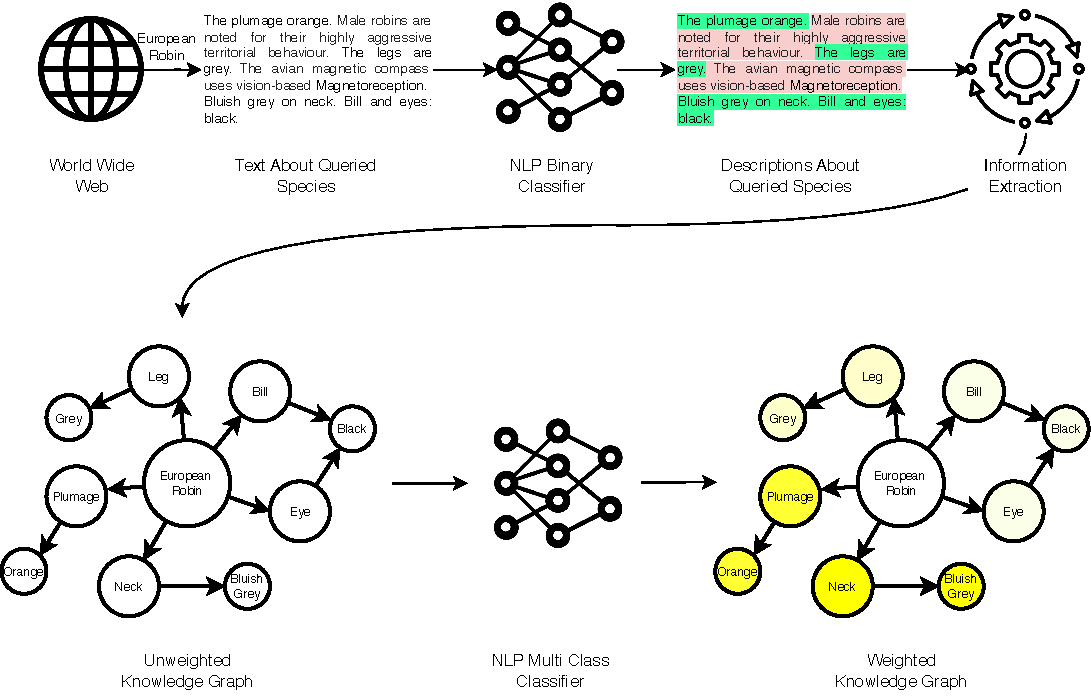
\includegraphics[width=1.25\textwidth]{workflow.pdf}}
    \caption{A simplified workflow. Text data is used to train a model to recognize species description. In this case the paragraph titles are used as labels. The model is deployed in a web crawler that searches the web for species description. These data are then used to train the NLP model independently of the visual-language hybrid model.}
    \label{fig:workflow}
\end{figure}


\subsection{Creation of the Dataset}
The World Wide Web has potentially an endless amount of species descriptions available.
However, this data is not structured and is certainly not in one place on the internet.
The web crawler needs to automatically query species description pages from search engines, search those queried pages for description text, and store the text that qualifies as a description.
Description sentences can be theoretically limitless, e.g. for a Brown Bear description text could be: "The fur is brown", "The brown bear has brown fur".
Sentences can also have a more difficult semantic, e.g. "The fur of the Brown bear is similar to that of the Grizzly bear".
It will not be feasible to use a classic machine learning approach that requires a rule-based match system for sentence classification. 
A DNN that can automatically extract the features and classify the text can help out.
This model will aim to assign labels to sentences, paragraphs or even complete documents. 
However, to properly train a deep learning model that can classify text data, a large, accurate and consistent labelled dataset is needed \autocite{munappy_data_2019}.
In Figure \ref{fig:workflow} a simplified version of the proposed workflow can be found.

Several structured web sources like \href{http://www.Wikipedia.com}{Wikipedia}, \href{https://birdsoftheworld.org}{Birds of the World} and \href{http://powo.science.kew.org/}{Plants of the World Online} will be used to create this dataset.
These websites do not contain labels but do contain paragraph titles like 'Habitat', 'Characteristics'. 
These titles can be used as labels for the scraped text (true in the case of 'Characteristics' and false in the case of 'Habitat').
Using paragraph titles as labels will result in mislabelled data; not every description text is used in a paragraph about descriptions and vice versa.
To compensate for this a loss of \textcite{reed_training_2015} will be implemented: \( Softloss(q, t) =  \sum_{k=1}^{L} [\beta t _k + (1- \beta )q _k]log(q _k) \).
If the model prediction reaches a set threshold (\(\beta)\), the prediction will be treated as correct and the loss will be calculated accordingly.
To increase non-description data, random Wikipedia pages that do not contain description data can be used.

Using a pre-trained model with word embeddings can help models achieve better results than models trained from scratch \autocite{mikolov_distributed_2013}.
The use of a pre-trained model is called transfer learning and could speed up the training process and increase the accuracy of the deep learning model.
The Bidirectional Encoder Representations from Transformers (BERT) by \textcite{devlin_bert_2019} is already trained on a large corpus of English words and can be used freely.
As text classification with two different outputs is a relatively simple task, a slimmed-down and faster version of BERT, called distilBERT from \textcite{sanh_distilbert_2020}, will be used as a pre-trained model.
\textcite{sun_how_2020} already investigated the best way to fine-tune BERT for text classification. 
Their findings will be used to build a model in PyTorch \autocite{paszke_pytorch_2019}.
%In their best runs they used one dropout layer (0.1) and two linear layers. 
%Their dropout layer and first linear layer (768\footnote{The output from the last hidden layer of BERT is a tensor of 768.}, 512) will be kept the same.
%The last linear layer will have its output changed to two as there are two different classes.
%The final activation function will be a log softmax function\footnote{In certain situation the log softmax is proven to be numerically more stable than softmax, by taken the exponent of the value it can be converted to normal prediction values.}
The model will be evaluated based on left out test set and a precision/recall plot will be used to assess the accuracy model on a test set. 
When the f1 score is at least 0.95, the model will be evaluated based on left-out, smaller structured datasets like \href{http://www.llifle.com/}{LLifle} and \href{https://www.worldagroforestry.org/}{AgroForestry} to see how well the model generalises.
When the results of the left-out datasets reach at least a f1 score of 0,90 the model will be deemed sufficient for the web crawler.
%To additionally asses the model, descriptions that are close to the threshold value of 0.5 will be labelled manually to assess the model.

When the results from the distilBERT descriptions classification model are proven to be sufficient, it will be used in the web crawler.
Websites can be automatically queried using different search engines like \href{www.google.com}{Google} and \href{www.bing.com}{Microsoft Bing}.
The Python packages Requests (HTML-based) and Selenium (Java-based) can be used in a script to query the search engines.
Queries could be constructed by using species names plus "description" or "diagnosis". 
The \href{https://www.ipni.org/}{International Plant Name Index} (IPNI) will be used to gather described plant species (1,3M+) and the \href{https://birdsoftheworld.org/bow/home}{Birds of the World} will be used to gather described bird species (10k+).
%It has yet to be seen which species/query is the best combination and yields the most relevant results.
%When the right species/query combination is found, it can iterate over the species names and return relevant web pages from the search engines.
Text from the returned pages needs to be broken down into chunks or sentences.
The trained classification model for descriptions can check if a text part is a prediction.
%Before using the trained model, the retrieved text from the web page needs to be cleaned and the text will be broken down into single sentences.
There is the possibility that websites use data from other websites.
If these websites are queried, predictions from both websites will be stored in the database.
Checking for sentence similarity will ensure the train and test data for the following models are disjoint.
The duplicate sentences can be dropped using the last hidden state of the model and creating a cosine matrix \autocite{reimers_sentence-bert_2019}.
The web crawler will be run for two weeks or whenever 75,000 species have at least 20 different descriptions or chunks.
If the 75,000 species are reached first, the remaining species that do not have 20 different descriptions will not be used.
If after two weeks of web crawling there are not 75,000 species with a description, the species that do have 20 descriptions will be used.
The remaining species description will be appended to the species corresponding family.

For extracting subject-predicate-object expressions from the data, the sentences that are qualified as descriptions will be used.
The sentences first need to be processed in a pre-trained NLP pipeline that can extract part-of-speech and dependencies.
SpaCy \autocite{honnibal_spacy_2020} is a python package that offers these kinds of pipelines and will be used for semantic triple extraction.
A rule-based system needs to be set up based on the dependencies and the part-of-speech values. 
It has to be seen how well this rule-based system generalises.
Some text is written down in proper English, but a lot is written down in telegram-style.
%Extracting semantic triples and feeding them to the next model will remove all bias and similarity in the sentences (artefacts, misspelt words etc.)
An example of a processed sentence with the SpaCy package can be found in Figure \ref{fig:PoS_example}.

\begin{figure} [t]
    \centering
    \vspace{0cm}
    \makebox[\textwidth][c]{\includesvg[inkscapelatex=false, width=1.25\textwidth]{PoS_example.svg}}
    \caption{An example of part of speech and dependency parsing for the sentence: "The Brown bear has long and sharp claws.". The arrows contain the dependency tags and the words contain the part of speech tags.}
    \label{fig:PoS_example}
\end{figure}

%As the labels are based on the paragraphs titles, all the text inside a paragraph would get the same label. 
\subsection{Infer Species on Partial Descriptions}
As the input data is text data, using a pre-trained model provides better results \autocite{devlin_bert_2019, sanh_distilbert_2020, mikolov_distributed_2013}.
For both architecture bases, a version (distilled or full version of BERT) will be used.
The first approach will make use of a soft max activation function as last layer.
With the first model, the hidden state layer will be connected to one or several linear layers and will end in a softmax activation function.
This last activation function will output a probability for the input data belonging to one of the classes.

%However, with so much classes the softmax activation function in combination with a cross entropy loss function might not be suitable.
%The model will be very expensive to train which such a large amount of output classes; It start with random guesses out of the 20,000 labels and needs to 'learn' the correct classes based on the loss that is returned.
%Another downside of the softmax activation is that is does not try to keep different labels as far apart as possible.
%With a fixed amount of classes this is not a problem.
The second approach will be metric learning that learns distances between labels.
Deep metric learning minimises the distance if it looks at the same label and maximises the distance between different labels.
Nowadays, a popular deep learning model for metric learning is a so-called Triplett network \autocite{hoffer_deep_2015}, and this model will also be used in this research.
This network involves three identical networks that are combined into one single loss output.
The output will produce a single distance cost function between three input labels.
Triplet loss \autocite{schroff_facenet_2015} will be used to compute the loss between the labels.
Triplet loss uses an anchor label, tries to push a similar label towards the anchor, and pushes a different label away, resulting in larger distances for different labels.
As the last hidden state of BERT already contains a matrix, this last hidden state will be used as a feature for the loss function to compute the distance between two matrices.
\textcite{musgrave_pytorch_2020} provide an open-source library built on PyTorch that provides a straightforward implementation of deep metric learning miners and algorithms.

%The goal for both models is not to reach a good accuracy, but to see if the predictions make sense, and to see on which points to model focuses.

There is no way to check the final results of the model as there is no ground truth data.
We can first statistically and visually asses the most important words used for the predictions. 
E.g. does the model focuses on punctuation or does it focuses on important verbs, nouns, adjectives or combinations of one of these.
For retrieving focus words used for making species predictions, different techniques can be used.
\textcite{vig_multiscale_2019} developed an open package that visualises the attentions in transformer networks like BERT.
Simple visualisation like occlusions sensitivity heat maps can track the change in the prediction by removing words one by one \autocite{fleet_visualizing_2014}.
The benefit of occluding is that it can be done posthoc on a trained model.
Another approach is using the gradients of the network, like SmoothGrad \autocite{smilkov_smoothgrad_2017} or using the integrated gradients \autocite{sundararajan_axiomatic_2017}.
With SmoothGrad, noise is added to the data multiple times, and the average gradients are calculated.
With integrated gradients, one searches for the parts where the derivative has the steepest slope (i.e. the most information is added).
Integrated gradients can be implemented very quickly by calling the gradients operator in PyTorch.
All these examples can be done a posteriori and do not require any modifications to the network architecture.

When the model uses important key words in the prediction, a small survey with an expert like a botanist to validate the models results is an option.
The model will be fed a custom text span that corresponds to a species seen by the network.
The botanist will be presented the same text span and has to predict the species.
Both results will be compared, in case the results differ, the botanist can see if the model made a decent prediction.
For example, if the input text corresponds to the description of a Black Spruce (Picea mariana), but it predicts a different Spruce (Pinaceae) the models made a decent prediction. 

\section{Feasibility \& Limitations}

\begin{figure} [t]
    \centering
    \vspace{1cm}
    \hspace{-1.3cm}
    \makebox[\textwidth][c]{\includesvg[inkscapelatex=false, width=1.25\textwidth]{schedule.svg}}
    \caption{Time Schedule}
    \label{fig:time_schedule}
\end{figure}

In Figure \ref{fig:time_schedule}, an overview of the most important milestone and processes can be found.
The start of this thesis is on July 15 2021.
Other research is also dependent on some data that will be created in this research.
By bringing the starting date forward, the other researchers can use the data earlier.

\subsection{Web Crawler}
The first step is to create a web crawler pipeline. 
For this, data needs to be scraped from structured sources.
Scarping is not a computationally expensive task and can be done on a personal computer running Python with some basic packages like BeautifulSoup and Selenium.
However, training the model that can recognise description spans is computationally expensive and needs to be done GPU with CUDA architecture.
As the WUR server is not available for students at the time of writing (\thedate), the deep learning model for description recognition will be trained on \href{https://colab.research.google.com/}{Google Colab Pro}. 
The model can be trained for multiple epochs by storing and reloading the model at each instance, even if the connection times out.
The dataset will be initialised at every instance, the same seed will be set to ensure the training, validation, and testing data stays the same.

The model will be deployed on a personal laptop to crawl through the web pages and store sentences that contain description data.
A possible risk is that the trained model will not generalise well and fails to recognise description sentences.
In this case, new data needs to be scraped manually to make sure the model will generalise better.
The time needed for the deployment might also disappoint, as the scraping is reliant on search engines.
If too much scrapings happens in a bit of time, the query might malfunction as this will be detected, malfunctioning might be prevented by using a custom agent header or a timer to limit the number of queries within a time frame.
The model might also require a lot of time to process the data depending on the returned results.
If the query returns a lot of websites, all of the text of these website has to be checked against the model to see if the text is a prediction.
This is the reason why the scraper will be run for a limited time of two weeks.
Data will be limited to plants and birds species and especially species available in the INPI and BoW databases.
When scraping the data, the crawler will start with the plant species that have a description available in the PoWO database. 
If the web scraper takes longer then 2 weeks and will be cut of, at least the species with a high description probability have been queried and searched by the model.


\subsection{Natural Language Processing Model}
The processes in this research are dependent on each other.
The database creation needs to be finished before the NLP model can be trained.
However, a pipeline that processes and loads the data can already be built with preliminary results from the web crawler.
Both models (metric and softmax) will be trained on the WUR server.
Otherwise, both models will be trained on Google Colab Pro.
This will take more time as each the GPU are shared across multiple users and every instance the data  and model have to be loaded.

There is no ground truth data available for the NLP model that has to infer species based on partial descriptions.
A classic split in train and test data will not work. 
This will result in species that the model cannot classify as they are never seen in the training data.
The first step for validating this model is therefore to see which words are important for the predictions.
When this the results of the retrieved key words are sufficient there is still no real validation for the NLP results.
In this case a experimental setup needs to be set up to test the model against a span of text that is never seen by the model, but corresponds to a species seen by the model.
In this case a botanist (or other expert that can identify species based on descriptions) needs to be found and willing to participate.

\printbibliography

\end{document}